\documentclass[english]{beamer}

\usepackage{babel}
\usepackage{fontspec}

\usepackage{microtype}

\usepackage{csquotes}

\usepackage{amssymb,amsmath}

\usepackage[
            backend=biber,
            style=numeric,
            isbn=false,
            doi=false
        ]{biblatex}

\addbibresource{sources.bib}

% Colors
\usepackage{xcolor}
\definecolor[named]{uboBlue}{cmyk}{1,.7,0,0}
\definecolor[named]{uboYellow}{cmyk}{0,.3,1,0}
\definecolor[named]{uboGrey}{cmyk}{0,0,.15,.55}

% Theme
\usetheme{metropolis}
\usefonttheme{professionalfonts}

\metroset{block=fill}
\setbeamercolor{title}{fg=uboBlue}
\setbeamercolor{subtitle}{fg=normal text.fg}
\setbeamercolor{title separator}{fg=uboYellow}
\setbeamercolor{frametitle}{bg=black!20!uboBlue}
\setbeamercolor{itemize item}{fg=uboBlue}
\setbeamercolor{enumerate items}{fg=uboBlue}
\setbeamercolor{block title}{bg=uboYellow}

\title{A introduction to multilinear maps and their attacks using the example of CLT13}
\author{Lukas Kempf}
\date{2021-12-10}

\newcommand*{\todo}[1]{\textcolor{red}{TODO:~#1}}

\usepackage{suffix}
\newcommand{\citeauthoryear}[1]{\citeauthor{#1} \citeyear{#1}}
\WithSuffix\newcommand\citeauthoryear*[1]{\citeauthor*{#1} \citeyear{#1}}

\newcommand*{\IN}{\mathbb{N}}
\newcommand*{\IZ}{\mathbb{Z}}

\usepackage{mathtools}
\DeclareMathOperator{\smod}{mod}
\DeclareMathOperator{\id}{id}
\DeclareMathOperator{\crt}{CRT}
\DeclareMathOperator{\diag}{diag}

\newcommand*{\crtp}[2][i]{\crt_{(p_{#1})}\left(\left[#2\right]\right)}

\usepackage{epsdice}
\newcommand*{\rand}{\mathrm{rand}}
\newcommand*{\rgets}{\xleftarrow{\rand}}

\newcommand*{\pubkey}{\mathrm{pubKey}}

\usepackage{hyperref}

\begin{document}
    \begin{frame}[plain]
        \titlepage
    \end{frame}
    \begin{frame}{Outline}
        \begin{itemize}
            \item Multilinear maps
            \item CLT13
            \item DH with CLT13
            \item Attacking CLT13
        \end{itemize}
    \end{frame}
    \begin{frame}{Diffie-Hellman key exchange}
        \setbeamercolor*{block title}{bg=uboGrey}
        Let $G$ be finite cyclic group with generator $g$.

        \begin{columns}[onlytextwidth, t]
            \column{0.45\linewidth}
            \begin{block}{Alice}
                Choose random $a \in \IN$. Broadcast $g^a$.
            \end{block}
            \column{0.45\linewidth}
            \begin{block}{Bob}
                Choose random $b \in \IN$. Broadcast $g^b$.
            \end{block}
        \end{columns}

        Shared key: $(g^b)^a = (g^a)^b$

        \pause\vspace{0.6cm}
        Attacker knows $g^a$ and $g^b$.

        $\Rightarrow$ Obtaining $g^{ab}$ from this must be hard (CDH assumption).

        \pause
        Alternative stronger assumption: Given $g^a$ and $g^b$ it must be hard to differentiate $g^{ab}$ from random (DDH assumption).
    \end{frame}
    \begin{frame}{Multilinear maps}
        \begin{definition}[Multilinear Map \citeauthoryear*{boneh2003applications}]
            A map $e: G_1^n \leftarrow G_2$ is a \emph{n-multilinear map} if it satisfies the following properties:
            \begin{enumerate}
                \item $G_1$ and $G_2$ are groups of the same prime order
                \item if $a_1,\dots ,a_n \in \IZ$ and $x_1, \dots, x_n \in G_1$ then
                    \begin{equation*}
                        e\left( x_1^{a_1}, \dots, x_n^{a_n} \right) = e(x_1, \dots, x_n)^{a_1\dots a_n}
                    \end{equation*}
                \item if $g \in G_1$ is a generator of $G_1$ then $e(g, \dots, g)$ is a generator of $G_2$.
            \end{enumerate}
        \end{definition}
    \end{frame}
    \begin{frame}{Why multilinear maps matter}
        \begin{itemize}
            \item DH key-exchange between multiple parties in one round~\cite*{boneh2003applications}.
            \item Existence of cryptographic multilinear maps linked to the existence of indistinguishability obfuscation~\cite*{albrecht2020multilinear}.
            \item Building block for time-lock encryption~\cite*{liu2018build}.
        \end{itemize}
    \end{frame}
    \begin{frame}{DH with multilinear maps}
        Let $e: G_1^n \leftarrow G_2$ be a $n$-multilinear map and $g$ a generator of $G_1$.

        Each of the $n+1$ parties chooses $a_i \in \IN$ and broadcasts $h_i = g^{a_i}$.

        \begin{multline*}
            e(h_2, \dots, h_{n+1})^{a_1} = e(h_1, h_3, \dots, h_{n+1})^{a_2} = \dots \\
            = e(h_1, \dots, h_n)^{a_{n+1}} = e(g, \dots, g)^{a_1 \cdots a_{n+1}}
        \end{multline*}

        \pause
        Security assumption: Given $g, g^{a_1}, \dots, g^{a_{n+1}} \in G_1$ it is hard to compute $e(g, \dots, g)^{a_1 \cdots a_{n+1}} \in G_2$ (MDH assumption).
    \end{frame}
    \begin{frame}{How to construct such maps?}
        \blockquote[\citeauthoryear*{boneh2003applications}][]{The central open problem posed in this paper is the construction of cryptographic multilinear map generators when $n > 2$.}
        \pause

        \blockquote[\citeauthoryear*{boneh2003applications}][]{We also give evidence that such maps might have to either come from outside the realm of algebraic geometry, or occur as \enquote{unnatural} computable maps arising from geometry.}
    \end{frame}
    \begin{frame}{Chinese remainder theorem}
        \begin{theorem}[Chinese remainder theorem over the integers]
            Let $\{p_1, \dots, p_n\}$ be pairwise coprime integers and $N = \prod_i^n$. Then there exists a ring isomorphism $\IZ_N \cong \IZ_{p_1} \times \dots \times \IZ_{p_n}$.
        \end{theorem}

        More concretely we have maps
        \begin{equation*}
            f : x \longmapsto (x \smod p_1, \dots, x \smod p_n)
        \end{equation*}
        and
        \begin{equation*}
            g : (x_1, \dots, x_n) \longmapsto \sum_{i=1}^n 1_{p_i}x_i
        \end{equation*}
        where $1_{p_i}$ is chosen so that $f\left(1_{p_i}\right)$ is 1 in exactly the i-th component and $f \circ g = \id$.

        Notation: $x = \crtp{x_i}$
    \end{frame}
    \begin{frame}{Graded encoding schemes}
        Basically: Encoding ring elements with noise.

        For every $r \in R$ and degree $n \in \IN$ we have multiple possible encodings $S^{(r)}_n$.

        Addition is possible: For $v_1 \in S^{(r_1)}_n$ and $v_2 \in S^{(r_2)}_n$ we have $v_1 + v_2 \in S^{(r_1 + r_2)}_n$.

        Multiplication is possible: For $v_1 \in S^{(r_1)}_{n_1}$ and $v_2 \in S^{(r_2)}_{n_2}$ we have $v_1 \cdot v_2 \in S^{(r_1 \cdot r_2)}_{n_1 + n_2}$ if $n_1 + n_2$ is small enough.
    \end{frame}
    \begin{frame}{CLT13 --- Idea}
        Section based on the paper of \citeauthoryear{cryptoeprint:2013:183}.

        \begin{itemize}
            \item Use CRT to hide computations in the smaller rings by doing them concurrently in the larger ring
            \item Generate $n$ primes $p_1, \dots, p_n$ for CRT and compute $x_0 \coloneqq \prod_i^n p_i$
            \item Generate \enquote{small} primes $g_1, \dots, g_n$
            \item Let $r_1, \dots, r_n$ be \enquote{small} integers
            \item Let $z$ be random integer
            \item Let $\kappa$ be max encoding level
        \end{itemize}

        Encoding of vector $m \in \IZ^n$ in level $k$:
        \begin{equation*}
            c \equiv \frac{r_i \cdot g_i + m_i}{z^k} \mod p_i
        \end{equation*}
    \end{frame}
    \begin{frame}{CLT13 --- Idea}
        \begin{equation*}
            c \equiv \frac{r_i \cdot g_i + m_i}{z^k} \mod p_i
        \end{equation*}

        Zero-test parameter:
        \begin{equation*}
            p_{zt} = \sum_{i=1}^n h_i \left(z^\kappa \cdot g_i^{-1} \smod p_i\right) \cdot \prod_{i' \neq i} p_{i'} \mod x_0
        \end{equation*}
        \pause
        Applying the zero-test to a $\kappa$-level encoding $c$:
        \begin{equation*}
            p_{zt} \cdot c = \sum_{i=1}^n h_i \left(r_i + m_i \cdot (g_i^{-1} \smod p_i)\right) \cdot \prod_{i' \neq i} p_{i'} \mod x_0
        \end{equation*}
    \end{frame}
    \begin{frame}{CLT13 --- Idea}
        \begin{equation*}
            c \equiv \frac{r_i \cdot g_i + m_i}{z^k} \mod p_i
        \end{equation*}

        Adding encodings:
        \begin{equation*}
            \frac{r_i \cdot g_i + m_i}{z^k} + \frac{r'_i \cdot g_i + m'_i}{z^k} \equiv \frac{(r_i + r'_i) \cdot g_i + m_i + m'_i}{z^k} \mod p_i
        \end{equation*}

        Multiplying encodings:
        \begin{equation*}
            \frac{r_i \cdot g_i + m_i}{z^k} + \frac{r'_i \cdot g_i + m'_i}{z^{k'}} \equiv \frac{r^\dagger_i \cdot g_i + m_i \cdot m'_i}{z^{k + k'}} \mod p_i
        \end{equation*}
    \end{frame}
    \begin{frame}{CLT13 --- Public key}
        8 different parameters dependent on security parameter.

        Notation: $\rand$ means random number of appropriate size.

        Public key $\pubkey$:
        \begin{itemize}
            \item $x_0$
            \item $p_{zt}$
            \item $\tau$ random level-1 encodings of zero $\{x_j\}$ meaning $x_j = \crtp{\frac{\rand g_i}{z}}$
            \item $n$ more random level-1 encodings of zero
            \item $\ell$ random level-0 encodings of random values $\{x'_j\}$ meaning $x'_j = \crtp{\rand g_i + \rand}$
            \item Level-1 encoding of 1 $y = \crtp{\frac{\rand g_i + 1}{z}}$
        \end{itemize}
    \end{frame}
    \begin{frame}{CLT13 --- More operations}
        $\mathbf{samp}(\pubkey)$: Pick random subset of $\{x'_j\}$ and add together.

        $\mathbf{enc}(\pubkey, c, k)$: Raise level-0 encoding $c$ to level $k$ by multiplying with $y^k$.

        $\mathbf{reRand}(\pubkey, c)$: Re-randomize level-1 encoding $c$ (simplified version). Add to $c$ sum of random subset of $\{x_j\}$.

        $\mathbf{isZero}(\pubkey, c)$: Test if level-$\kappa$ encoding $c$ is zero (simplified version) by checking if $c \cdot p_{zt}$ is small enough.

        $\mathbf{ext}(\pubkey, c)$: Collect most significant bits of $c \cdot p_{zt}$ (simplified version).
    \end{frame}
    \begin{frame}{DH with CLT13}
        Key exchange between $\kappa + 1$ parties.

        Each party $i$: Let $a_i = \mathbf{samp}(\pubkey)$ be secret random value and broadcast
        \begin{equation*}
            h_i = \mathbf{reRand}(\pubkey, \mathbf{enc}(\pubkey, a_i, 1))
        \end{equation*}

        Shared encoding:
        \begin{equation*}
            a_1 h_2 \dots h_{\kappa+1} = h_1 a_2 h_3 \dots h_{\kappa+1} = \dots = h_1 \dots h_{\kappa} a_{\kappa + 1}
        \end{equation*}

        Shared value can be obtained by extraction.
    \end{frame}
    \begin{frame}{CLT13 --- Hardness assumption}
        \begin{definition}[Graded Descicional Diffie-Hellman (GDDH)]
            Consider following process:
            \begin{enumerate}
                \item Generate a public key $\pubkey$ with security parameter $\lambda$
                \item Choose $a_j = \mathbf{samp}(\pubkey)$ for all $1 \leq j \leq \kappa + 1$
                \item Set $u_j = \mathbf{reRand}(\pubkey, \mathbf{enc}(\pubkey, 1, a_j))$ for all $1 \leq j \leq \kappa + 1$
                \item Choose $b = \mathbf{samp}(\pubkey)$
                \item Set $v = \mathbf{reRand}(\pubkey, \mathbf{enc}(\pubkey, \kappa, \prod_{i=1}^{\kappa + 1} a_i))$
                \item Set $w = \mathbf{reRand}(\pubkey, \mathbf{enc}(\pubkey, \kappa, b))$
            \end{enumerate}

            The GDDH assumption states that an attacker with runtime polynomial in $\lambda$ has only negligible chance to differentiate $v$ and $w$ given the $u_j$ and $\pubkey$.
        \end{definition}
    \end{frame}
    \begin{frame}{Attacking CLT13 --- CRT-ACD}
        Section based on the paper of \citeauthoryear{cryptoeprint:2014:906}.
        \begin{definition}[CRT-ACD Problem]
            Let $n, \eta, \varepsilon \in \IN$. Let $\chi_\varepsilon$ be distribution over $(-(2^\varepsilon), 2^\varepsilon) \cap \IZ$. For given $\eta$-bit primes $p_1, \dots, p_n$ define
            \begin{equation*}
                D_{\chi_\varepsilon, \eta, n}(p_1, \dots, p_n) = \left\lbrace \crtp{r_i} \mid r_i \rightarrow \chi_\varepsilon \right\rbrace.
            \end{equation*}
            CRT-ACD Problem: Given many samples from $D_{\chi_\varepsilon, \eta, n}(p_1, \dots, p_n)$ and $x_0 = \prod_{i=1}^n p_i$ find all $p_i$.
        \end{definition}
        \pause

        Let $\hat{p}_i = x_0 / p_i$. $\hat{P} = \crtp{\hat{p}_i}$ is called auxillary input.
    \end{frame}
    \begin{frame}{Attacking CLT13 --- CRT-ACD}
        \begin{lemma}
            Given $a = \crtp{r_i} \rightarrow D_{\chi_\varepsilon, \eta, n}(p_1, \dots, p_n)$ and $\hat{P} = \crtp{\hat{p}_i}$ it holds that
            \begin{equation*}
                \hat{P} \cdot a \smod x_0 = \crtp{\hat{p}_i \cdot r_i} = \sum_{i=1}^n \hat{p}_i \cdot r_i
            \end{equation*}
            if $\varepsilon + \log n + 1 < \eta$.
        \end{lemma}
        \pause
        Sketch of proof: Consider second equation modulo $p_i$. Ensure that left side is smaller that $x_0$. Result follows from uniqueness of CRT.
    \end{frame}
    \begin{frame}{Attacking CLT13 --- CRT-ACD}
        Let $a = \crtp{a_i}$, $b = \crtp{b_i}$. Assume lemma is applicable:
        \begin{equation*}
            ab\hat{P} \smod x_0 = \sum a_i b_i \hat{p}_i
        \end{equation*}
        \pause

        As matrix equation:
        \begin{equation*}
            ab\hat{P} \smod x_0 =
            \begin{pmatrix}
                a_1 & a_2 & \cdots & a_n
            \end{pmatrix}
            \begin{pmatrix}
                \hat{p}_1 & 0 & \cdots & 0 \\
                0 & \hat{p}_2 & \cdots & 0 \\
                0 & 0 & \ddots & 0 \\
                0 & 0 & \cdots & \hat{p}_n
            \end{pmatrix}
            \begin{pmatrix}
                b_1 \\
                b_2 \\
                \vdots \\
                b_n
            \end{pmatrix}
        \end{equation*}
    \end{frame}
    \begin{frame}{Attacking CLT13 --- CRT-ACD}
        Collecting more samples ($1 \leq i,j \leq n$):
        \begin{equation*}
            a_i = \crtp[k]{a_{k, i}}, b = \crtp[k]{b_k}, c_j = \crtp[k]{c_{k, j}}
        \end{equation*}

        Stating matrix equations:
        \begin{equation*}
            w_{i,j} =
            \begin{pmatrix}
                a_{1, i} & a_{2, i} & \cdots & a_{n, i}
            \end{pmatrix}
            \begin{pmatrix}
                b_1 \hat{p}_1 & 0 & \cdots & 0 \\
                0 & b_2 \hat{p}_2 & \cdots & 0 \\
                0 & 0 & \ddots & 0 \\
                0 & 0 & \cdots & b_n \hat{p}_n
            \end{pmatrix}
            \begin{pmatrix}
                c_{1, j} \\
                c_{2, j} \\
                \vdots \\
                c_{n, j}
            \end{pmatrix}
        \end{equation*}
        \begin{equation*}
            w'_{i,j} =
            \begin{pmatrix}
                a_{1, i} & a_{2, i} & \cdots & a_{n, i}
            \end{pmatrix}
            \begin{pmatrix}
                \hat{p}_1 & 0 & \cdots & 0 \\
                0 & \hat{p}_2 & \cdots & 0 \\
                0 & 0 & \ddots & 0 \\
                0 & 0 & \cdots & \hat{p}_n
            \end{pmatrix}
            \begin{pmatrix}
                c_{1, j} \\
                c_{2, j} \\
                \vdots \\
                c_{n, j}
            \end{pmatrix}
        \end{equation*}
    \end{frame}
    \begin{frame}{Attacking CLT13 --- CRT-ACD}
        \begin{equation*}
            w_{i,j} =
            \begin{pmatrix}
                a_{1, i} & a_{2, i} & \cdots & a_{n, i}
            \end{pmatrix}
            \begin{pmatrix}
                b_1 \hat{p}_1 & 0 & \cdots & 0 \\
                0 & b_2 \hat{p}_2 & \cdots & 0 \\
                0 & 0 & \ddots & 0 \\
                0 & 0 & \cdots & b_n \hat{p}_n
            \end{pmatrix}
            \begin{pmatrix}
                c_{1, j} \\
                c_{2, j} \\
                \vdots \\
                c_{n, j}
            \end{pmatrix}
        \end{equation*}

        Collecting $w_{i,j}$ and $w'_{i,j}$ into matrices $\mathbf{W}$ and $\mathbf{W'}$:
        \begin{align*}
            \mathbf{W} &= \mathbf{A}^T \cdot \diag(b_1 \hat{p}_1, \dots, b_n \hat{p}_n) \cdot C \\
            \mathbf{W'} &= \mathbf{A}^T \cdot \diag(\hat{p}_1, \dots, \hat{p}_n) \cdot C
        \end{align*}

        \pause
        Assume $\mathbf{A}$ and $\mathbf{C}$ are invertible:
        \begin{equation*}
            \mathbf{W} \cdot \mathbf{W'}^{-1} = \mathbf{A}^T \cdot \diag(b_1, \dots, b_n) \cdot \mathbf{A}^{T^{-1}}
        \end{equation*}
    \end{frame}
    \begin{frame}{Attacking CLT13 --- CRT-ACD}
        \begin{equation*}
            \mathbf{W} \cdot \mathbf{W'}^{-1} = \mathbf{A}^T \cdot \diag(b_1, \dots, b_n) \cdot \mathbf{A}^{T^{-1}}
        \end{equation*}

        Calculating eigenvalues of $\mathbf{W} \cdot \mathbf{W'}^{-1}$ yields $B = \{b_1, \dots, b_n\}$.

        \pause
        Assume are $b_i$ pairwise distinct:
        \begin{equation*}
            \gcd(b - b_i, x_0) = p_i
        \end{equation*}
    \end{frame}
    \begin{frame}{Attacking CLT13 --- Adapting the attack}
        Recall:
        \begin{equation*}
            p_{zt} = \sum_{i=1}^n h_i \left(z^\kappa \cdot g_i^{-1} \smod p_i\right) \cdot \prod_{i' \neq i} p_{i'} \mod x_0
        \end{equation*}

        \pause
        Let $a = \crtp{r_i g_i / z^\kappa}$ be top-level encoding of 0.
        \begin{equation*}
            p_{zt} \cdot a \smod x_0 = \crtp{\hat{p}_i h_i r_i} = \sum_{i = 1}^n \hat{p}_i h_i r_i
        \end{equation*}

        \pause
        We get similar attack by spanning
        \begin{equation*}
            x'_j \cdot x'_1 \cdot x_k \cdot y^{\kappa - 1} \cdot p_{zt} \smod x_0 \text{ and } x'_j \cdot x_k \cdot y^{\kappa - 1} \cdot p_{zt} \smod x_0
        \end{equation*}
        for $1 \leq j,k \leq n$.
    \end{frame}
    \begin{frame}{Current state}
        \todo{Slide really needed? Or just link to website? Or just CLT type constructions?}
        CLT13 and improvement CLT15 broken in regards to GDDH~\cite{cryptoeprint:2014:906,cryptoeprint:2016:135}. iO based on CLT13 has been broken in multiple cases~\cite*{cryptoeprint:2019:1254,cryptoeprint:2019:309}.

        MZ17 (based on CLT13) is still standing regarding the GDDH assumption~\cite{cryptoeprint:2017:946}.

        Lattice based approaches have been successfully attacked regarding GDDH and iO.

        More (partially outdated) info: \url{https://malb.io/are-graded-encoding-schemes-broken-yet.html}
    \end{frame}
    \begin{frame}{Why this topic?}
        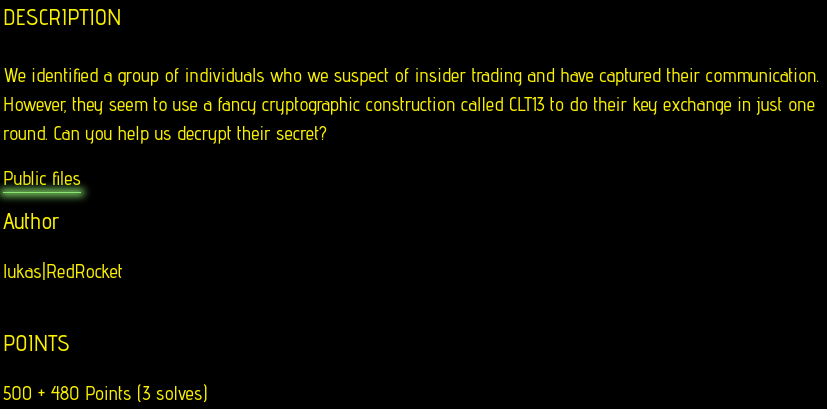
\includegraphics[width=\linewidth]{img/chall_desc.png}
    \end{frame}
    \begin{frame}[allowframebreaks]{References}
        \printbibliography[heading=none]
    \end{frame}
\end{document}